\section[Historia]{Historia języka andro}

\begin{spacing}{1.1}
Na planecie Maŕid, na której znajduje się Cesarstwo And́royas istnieje szereg
głównych rodzin językowych:

\begin{itemize}
    \item kaireńskie (lono, wekański, izolski, amharyjski, teoński, lideski),
    \item keilijskie (achab, esocki, mapelski, vireński, chizelski, ichepski,
    esrański),
    \item nahadyjskie (rilla, chopejski, nahadyjski),
    \item nenneckie (wczesnonennecki, osuński, tiharski, staronennecki,
    androyasański cesarski, doryjski, faryjski, nomisrański, andro),
    \item papityjskie (papityjski, betulski, resirski),
    \item turańskie (wczesnoagavański, isiski, chicha, wczesnoturański, ghia,
    turański),
    \item fetuckie (wczesnofetucki, imfuvo, farandyjski),
    \item nagiryjskie (alnogh, kharski, lirtycki, chojit, jizivański),
    \item południowe (jerebski, woymnar, papedyjski, alimuno, maddyjski)
\end{itemize}

Najwcześniejsze zabytki językowe, które udało się odkryć, to pismo kahejskie na 
glinianych tablicach sprzed około 5000 lat przed Zjednoczeniem.

Język \emph{andro} znany jest również jako język androyasański (\emph{Inrat yi
Androyas}), i wywodzi się z języka androyasańskiego cesarskiego (zwanego również
cesarskim) (\emph{eygepa inrat}).

Język androyasański cesarski był językiem częściowo sztucznym. Powstał na
podstawie języka handlarzy używanego w~kontaktach pomiędzy Królestwem Nennek,
a~krajami Zachodu i~został zaproponowany jako drugorzędny język urzędowy po
powstaniu Drugiego Cesarstwa. Łącząc cechy języka staronenneckiego,
kaireńskiego, keilijskiego i~turańskiego wydawał się idealnym kandydatem na
język zjednoczonych krajów.

Androyasański cesarski był krytykowany ze względu na istnienie tam bardzo 
silnego związku z~językiem nenneckim, co powodowało pewne trudności: na przykład 
w~zapisie w~sylabicznym piśmie chizelskim. Jednak po upadku Drugiego Cesarstwa 
już był rozpowszechniony jako język warstw wyższych i~stawał się narzędziem 
uniwersalnej komunikacji, a~potem ewoluował jak każdy język naturalny.

Współczesny \emph{andro} różni się od języka cesarskiego między innymi utratą
formy czasu przyszłego na rzecz partykuły \emph{ze}, zmianą formy użycia
partykuł \emph{do} oraz \emph{hemi}, utratą głoski [y], geminantów [rr] i [pp]
i~szeregiem innych zmian fonetycznych.

Od powstania Trzeciego Cesarstwa, a~także poprzez wpływ Cesarstwa, jest jedynym
językiem, który jest znany na wszystkich Wyspach i~jest nauczany we wszystkich
krajach, włączając z~w to Wolne Stany Ezimruk. Począwszy od początku VII wieku
po Zjednoczeniu, Republika Nennek nie uczy już powszechnie języka nenneckiego
w~szkołach, zastąpiwszy go tylko i~wyłącznie \emph{andro} oraz turańskim.

Do zapisu języka używa się trzech głównych sposobów -- zapisu
ideograficzno-sylabicznego, tzw. nowoczesnego (\emph{nu͞er isdara͞o huark} --
dosłownie,,nowe podzielone słowa''), zapisu sylabiczno-fonetycznego, tzw.
południowego (\emph{pantyi aysiji} -- dosłownie ,,południowe znaki'') oraz
alfabetów fonetycznych, takich jak \emph{chiwo}.

\subsection{Alfabet fonetyczny \emph{chiwo}}

Alfabet fonetyczny ma 27 znaków i nie rozróżnia wielkości znaków.

\emph{chiwo} w wersji odręcznej, może wyglądać w następujący sposób:

\begin{center}
    
\includegraphics[width=5cm]{katia-signature.png}    
\end{center}

Jest to odręczny zapis imienia \emph{Katia}, ręką samej cesarzowej,
\textbf{Katii mal Arkai}. Jej mąż, \textbf{So'tak mal Valor}, podpisuje się 
następująco:

\begin{center}
    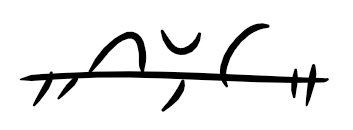
\includegraphics[width=5cm]{sotak.png}
\end{center}

Zapis w alfabecie fonetycznym, z wykorzystaniem specjalnego kroju \emph{desaho},
przeznaczonego do pisania znaków drogowych, informacji turystycznej i innych
informacji publicznych wygląda następująco:

\begin{center}
    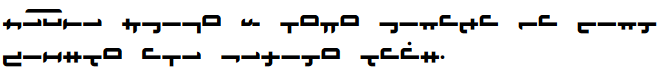
\includegraphics[width=12cm]{desaho.png}
\end{center}

\note{Tekst ten, \emph{ze͞uye chido yi boso hinaja va fint wirklo abe gepito laák}
nie ma większego sensu, ale jest to pangram -- używany jako odpowiednik
polskiego ,,pchnąć w tę łódź jeża lub ośm skrzyń fig''.}
\skipline

Ten sam tekst z wykorzystaniem popularnego kroju wzorowanego na piśmie
odręcznym, Na͞epo:

\begin{center}
    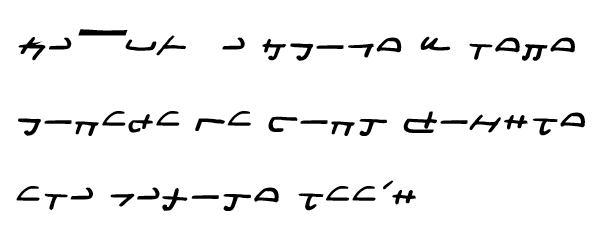
\includegraphics[width=12cm]{naepo.png}
\end{center}

W 2007 roku zaproponowana została transkrypcja androyasańskiego do alfabetu 
łacińskiego (transkrypcja Kadala), poprawiona w~latach 2013 (transkrypcja 
ZSC) i ostatecznie ustalona rok później (transkrypcja Ziri). W~tym słowniku
używana jest tylko i~wyłącznie transkrypcja Ziri.

Język nie jest całkowicie jednorodny -- jako, że włada nim ponad miliard 
użytkowników, pojawiają się w~nim dialekty oraz zachowania i~zasady specyficzne 
dla danej kultury lub regionu. 

Ten słownik skupiać się będzie na literackiej formie języka androyasańskiego,
nazywanej \emph{ardo andro} (wysoki androyasański), pewne uwagi dotyczące
dialektów będą zawarte w~dodatkowych opisach do haseł.

\end{spacing}